\section{Introducción}

El grafeno es uno de los materiales que más ha sido investigado en las últimas décadas y que más atención ha recibido desde su popularización tras su síntesis en 2004 llevada a cabo por primera vez por Geim y Novoselov \cite{science2004}, lo cual les llevaría a recibir el premio Nobel años más tarde. Debido a esta fama, muchos de mi generación, yo incluido, escuchamos su nombre por primera vez en el instituto, seguido de una charla sobre sus muchas y extraordinarias propiedades, simplificadas en gran medida para la comprensión de un adolescente. No obstante, la promesa de innovación tecnológica captó el interés de muchos de nosotros y ha llevado al estudio exhaustivo de este material y la publicación de incontables artículos explorando todas sus posibles aplicaciones; además de dar cabida a multitud de trabajos de final de carrera, como este. \\

Su nombre, acuñado por primera vez en 1986 \cite{BOEHM1986241}, hace referencia a una capa singular de grafito, uno de los muchos materiales alótropos del carbono y que se encuentra abundantemente en la naturaleza y, como caso particular, en las minas de nuestros lápices. Esta monocapa de grafito mantiene una estructura hexagonal o de panal con distancia de aproximadamente $0.142$ nm (o $1.42$ \AA) entre átomos de carbono. Esto se permite gracias a una hibridación de tipo $sp^2$ producida en los orbitales $s$ y $p$ del carbono, que dota a los átomos de una estructura triangular plana, formando enlaces covalentes de tipo $\sigma$ entre ellos. Estos enlaces de tipo $\sigma$ son los que acaban confiriendo al grafeno una gran fortaleza y rigidez, superior a la de cualquier otro material medido, como se vio experimentalmente en 2008 al fijar el módulo de Young del grafeno en $1.0 \pm 0.1 $ TPa \cite{science}. El grafeno también exhibe propiedades electrónicas exóticas, como un gap de semiconductor nulo (densidad de estados nula en el nivel de Fermi). Esta anulación exacta en el nivel de Fermi tiene como consecuencia una relación de dispersión lineal a bajas energías, determinando una región conocida como los \emph{conos de Dirac} (ver Figura \ref{fig:4.0}), en los cuales los electrones, en la banda de conducción, y huecos, en la banda de valencia, se comportan como fermiones relativistas sin masa (o fermiones de Dirac) \cite{castro-neto}. \\
\vspace{-.5cm}
\begin{figure}[!h]
    \centering
    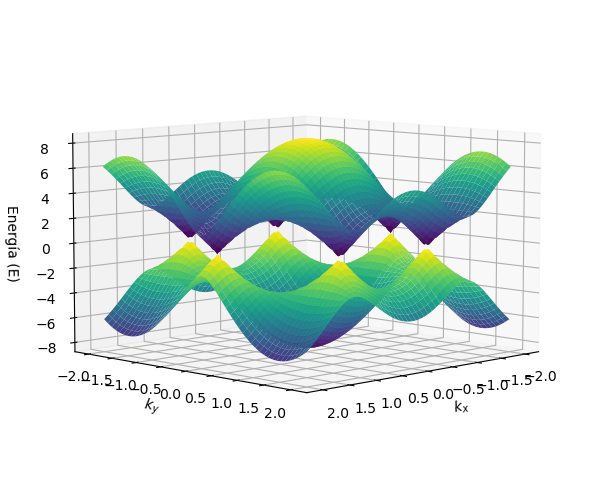
\includegraphics[width = .6\linewidth]{ADJUNTOS/conos-dirac.png}
    % \vspace{-.7cm}
    \caption{Relación de dispersión del grafeno $E(\B{k})$ y conos de Dirac. }
    \label{fig:4.0}
\end{figure}
% No obstante, a pesar de tener una gran cantidad de propiedades, el grafeno presenta un gap nulo de semiconductor, lo que impide poder usarlo en electrónica para la elaboración de circuitos.\\

% Como se ha demostrado en multitud de estudios, una posibilidad para abrir el gap dentro del grafeno puede ser inducir estrés mecánico estirando el grafeno. La ruptura de simetría de la red hexagonal puede modificar la relación de dispersión en los puntos de Dirac, dándonos resultados 

En este trabajo estudiamos las propiedades mecánicas del grafeno, además de explorar la posibilidad de modificar las propiedades electrónicas del grafeno, mediante el estiramiento de la red en la dirección \emph{armchair} (ver Figura \ref{fig:1.1}). Bajo diferentes técnicas de estiramiento y modificando de forma selectiva la red con otros elementos químicos o con defectos estructurales, podremos no sólo cuantificar y comprender mejor las propiedades mecánicas del grafeno sino también la respuesta de romper la simetría hexagonal de la red. Como veremos más adelante, estirar nos permitirá estimar las constantes elásticas del grafeno y conllevará a cambios en la estructura y su estabilidad y en las propiedades electrónicas en determinadas zonas de la red, como se ha comprobado extensamente en experimentos y simulaciones numéricas \cite{PhysRevB.81.241412} \cite{MEMARIAN2015348}\cite{LOPEZPOLIN201742} . \\

\begin{figure}[htbp]
    \centering
    \def\svgwidth{.4\textwidth}
    \input{armchair-zigzag.pdf_tex}
    \caption{Grafeno y las direcciones \emph{armchair} y \emph{zigzag}. }
    \label{fig:1.1}
\end{figure}

Para entender este cambio de las propiedades electrónicas del grafeno, utilizaremos la \textbf{Teoría del Funcional de la Densidad} (\emph{Density Functional Theory}, DFT) a través de simulaciones numéricas. La DFT \cite{sholl} es una teoría usada ampliamente en el ámbito de la física-química e ingeniería para el cálculo de las propiedades electrónicas de un conjunto de átomos como una molécula o parte de una estructura cristalina. En concreto, la DFT se basa en un método variacional que busca la minimización de la energía del estado fundamental del sistema de átomos y electrones por medio de dos teoremas matemáticos fundamentales de la mecánica cuántica aplicada a la física de la materia condensada, conocidos como los \textbf{Teoremas de Hohenberg y Kohn}, que permiten simplificar la ecuación de Schrödinger del sistema de manera significativa. Estos teoremas se estudiarán en las siguientes secciones, así como el código de simulación (FIREBALL) de DFT y sus correspondientes aproximaciones.\\
